\chapter{GitHub Pagesの設定(デプロイをする)}
\section{gitmodulesの設定}

  \begin{tcolorbox}[title=gitmodulesとは]
    Git サブモジュールは、あるリポジトリの内容を別のリポジトリ内に含めることを、参照されるリポジトリの場所を指定するだけでできるようになる Git SCMの機能です。 
    
    これは、外部ライブラリのソースをアプリケーションのソースツリーに含めるメカニズムを提供します。
    引用:\url{https://devcenter.heroku.com/ja/articles/git-submodules#:~:text=Git%20%E3%82%B5%E3%83%96%E3%83%A2%E3%82%B8%E3%83%A5%E3%83%BC%E3%83%AB%E2%80%8B%E3%81%AF,%E3%83%A1%E3%82%AB%E3%83%8B%E3%82%BA%E3%83%A0%E3%82%92%E6%8F%90%E4%BE%9B%E3%81%97%E3%81%BE%E3%81%99%E3%80%82}

  \end{tcolorbox}

  ということで、デプロイする時に、この設定をしないとエラーが発生するので、設定をしましょう

  \begin{shaded}
    \begin{verbatim}
    $ touch .gitmodules
    \end{verbatim}
  \end{shaded}

  \begin{figure}[H]
    \centering
    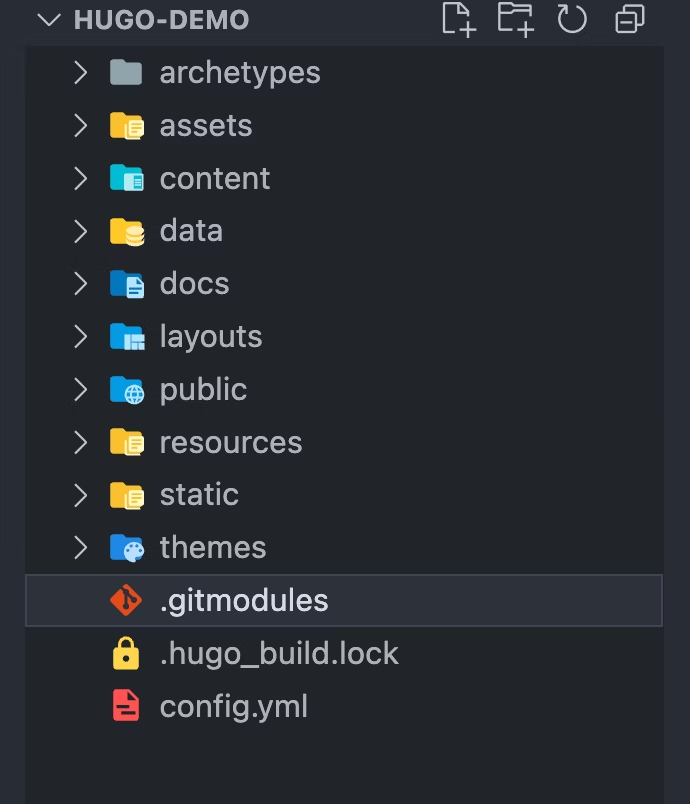
\includegraphics[width=8cm]{./image/02-chap6/make-modules-tree.png}
    \caption{GitModuleを作った時のTree構造}
    \label{chap6-make-modules-tree-image}
  \end{figure}

  テーマによって、設定内容が変わってくるので、テーマに合わせた設定にしてください。

  \begin{tcolorbox}[breakable]
    \begin{verbatim}
      [submodule "themes/hugo-theme-stack"]
      path = themes/hugo-theme-stack
      url = https://github.com/CaiJimmy/hugo-theme-stack
    \end{verbatim}
  \end{tcolorbox}

\section{baseurlの設定}

  あとはbaseURLを指定しましょう。
  ここが正しくないと、CSSがうまいこと読み取られないなどのバグが発生します。

  ということで、configファイルを編集しましょう。

  今回は、自分の設定をそのまま表示させていますが、カスタムドメインを使っていない場合は、https://GitHubのユーザー名.github.io/レポジトリ名/と設定しましょう。
  カスタムドメインを使用している場合は、設定したドメインをそのまま書き込んでください。

  \begin{tcolorbox}[breakable]
    \begin{verbatim}
      baseURL: "https://harutiro.github.io/hugo_test_qiita/"
      languageCode: ja
      title: My New Hugo Site
      theme: hugo-theme-stack
      publishDir: "docs"

      menu:
          main:
            - identifier: home
              name: Home
              url: /
              params:
                icon: home
    \end{verbatim}
  \end{tcolorbox}

\section{静的なファイルを生成する}

  それでは、GitHub Pagesの公開をするために、静的なファイルを生成します。
  生成する時にdocsに作ってもらえると都合がいいので、configを設定しておきましょう。

  publishDir: "docs"を追記してあげてください。

  \begin{tcolorbox}[breakable]
    \begin{verbatim}
      baseURL: ""
      languageCode: ja
      title: My New Hugo Site
      theme: hugo-theme-stack
      publishDir: "docs"

      menu:
          main:
            - identifier: home
              name: Home
              url: /
              params:
                icon: home
    \end{verbatim}
  \end{tcolorbox}


  あとは下記のコマンドを打ち込んで静的なファイル(html,cssなど)を作成しましょう


  \begin{shaded}
    \begin{verbatim}
    $ hugo
    \end{verbatim}
  \end{shaded}

  \begin{figure}[H]
    \centering
    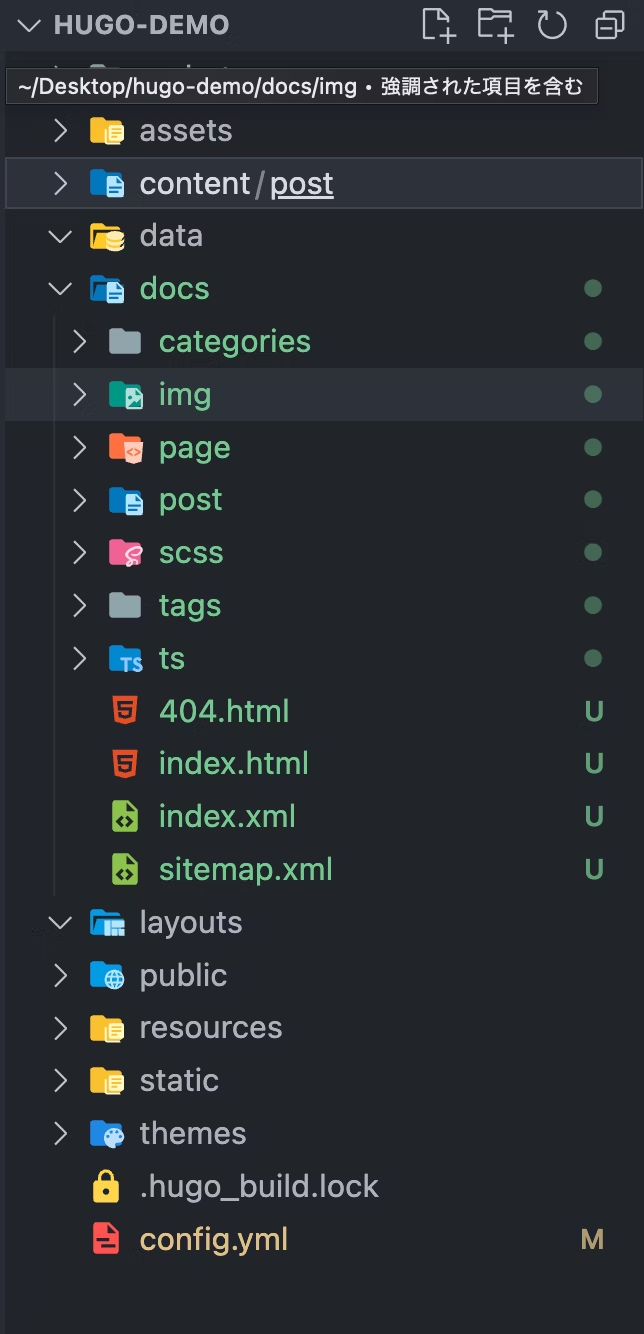
\includegraphics[width=6cm]{./image/02-chap6/docs-genelate.png}
    \caption{docsに静的なファイルが生成された図}
    \label{chap6-docs-genelate-image}
  \end{figure}

\section{GitHub Pagesの設定をする}

  それでは、GitHubを用いてデプロイを行ってみましょう。
  とりあえず、いつもの手順でGitHubに公開しましょう。

  \begin{shaded}
    \begin{verbatim}
    $ git init
    $ git add -A
    $ git commit -m "initalCommit"
    $ git remote add origin 個人のレポジトリ
    $ git push origin master
    \end{verbatim}
  \end{shaded}

  \begin{figure}[H]
    \centering
    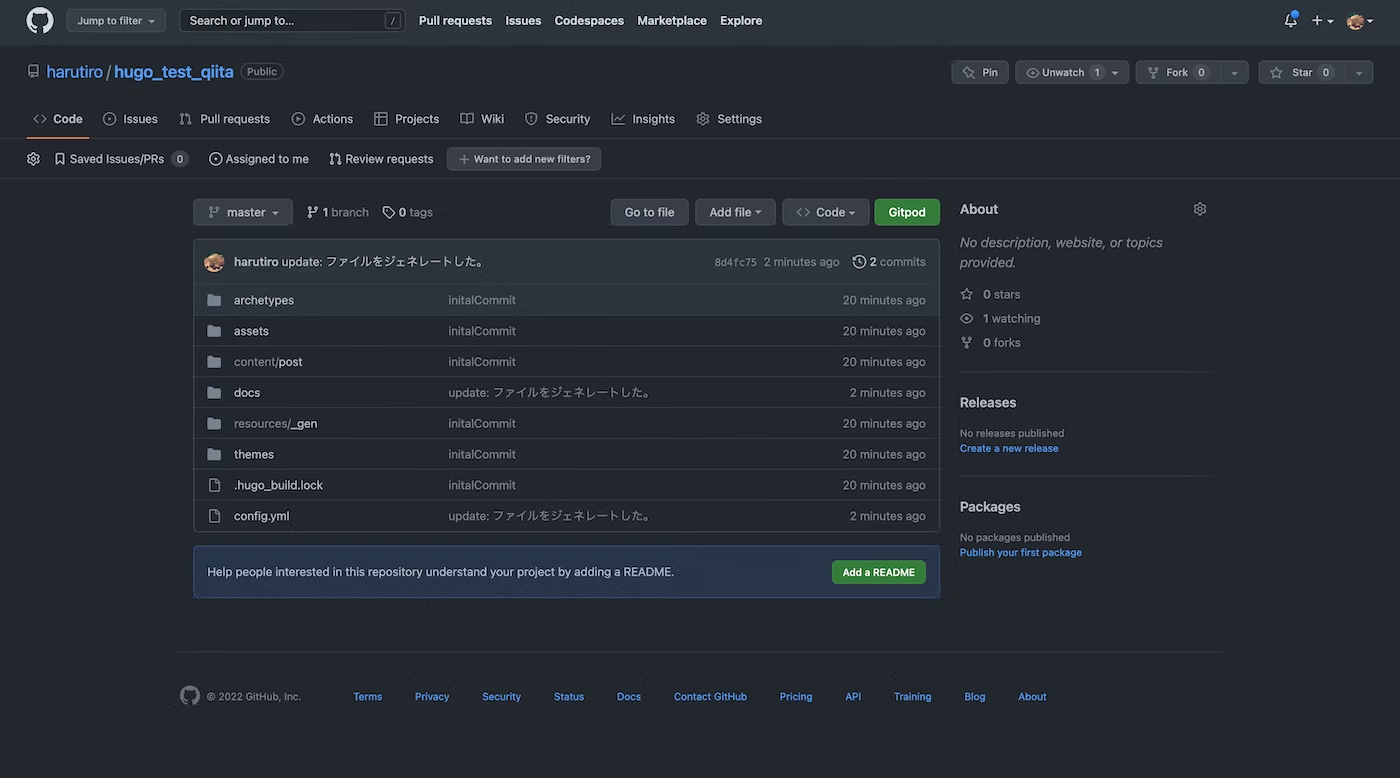
\includegraphics[width=8cm]{./image/02-chap6/git1.png}
    \caption{レポジトリが作成された様子}
    \label{chap6-git1-image}
  \end{figure}

  それでは、pagesの設定をしていきましょう。
  setting/pagesを開きましょう。

  \begin{figure}[H]
    \centering
    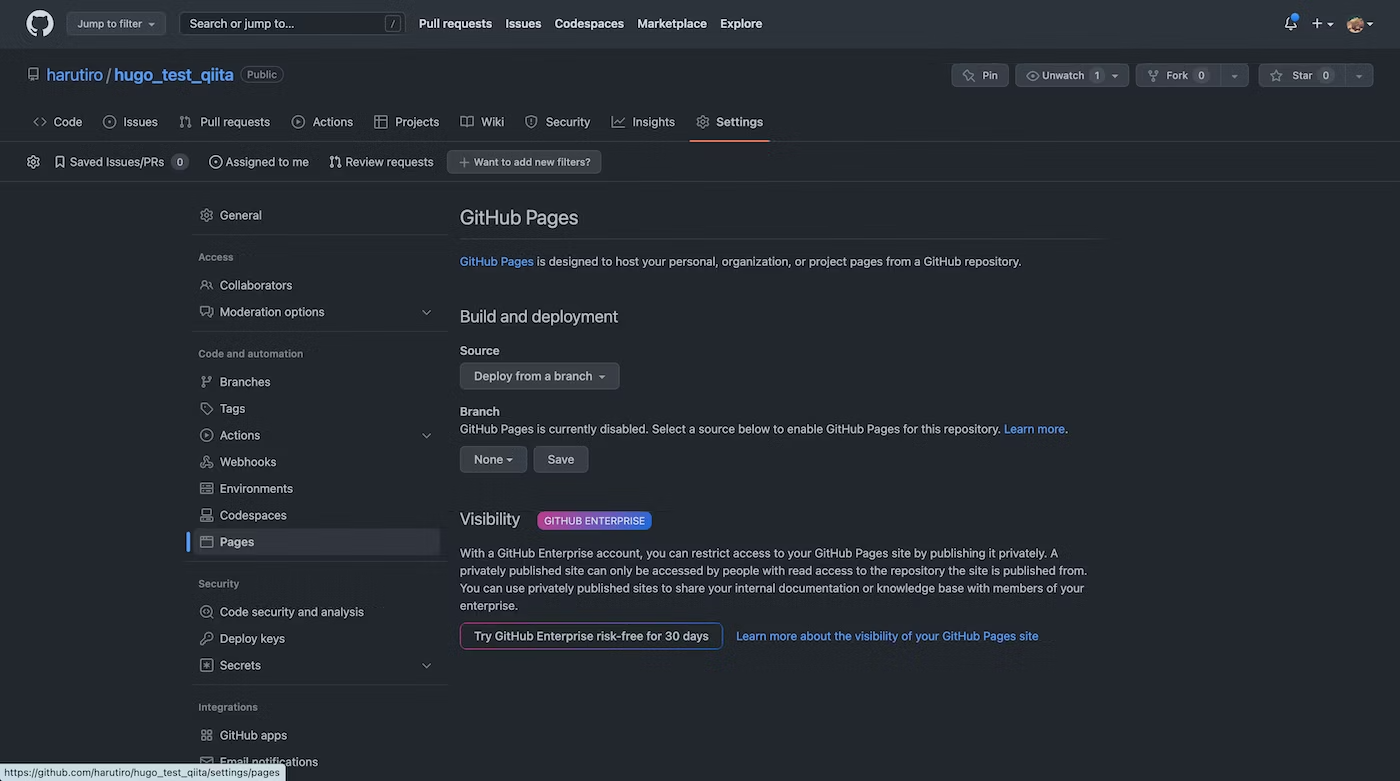
\includegraphics[width=8cm]{./image/02-chap6/git2.png}
    \caption{pagesの設定画面}
    \label{chap6-pages1-image}
  \end{figure}

  sourceをDeploy from a branchに設定して
  Branchをmaster /docsに設定しましょう

  カスタムドメインは今回は説明しません。
  これで、masterにデプロイして、しばらく待つとデプロイが始まります。

  \begin{figure}[H]
    \centering
    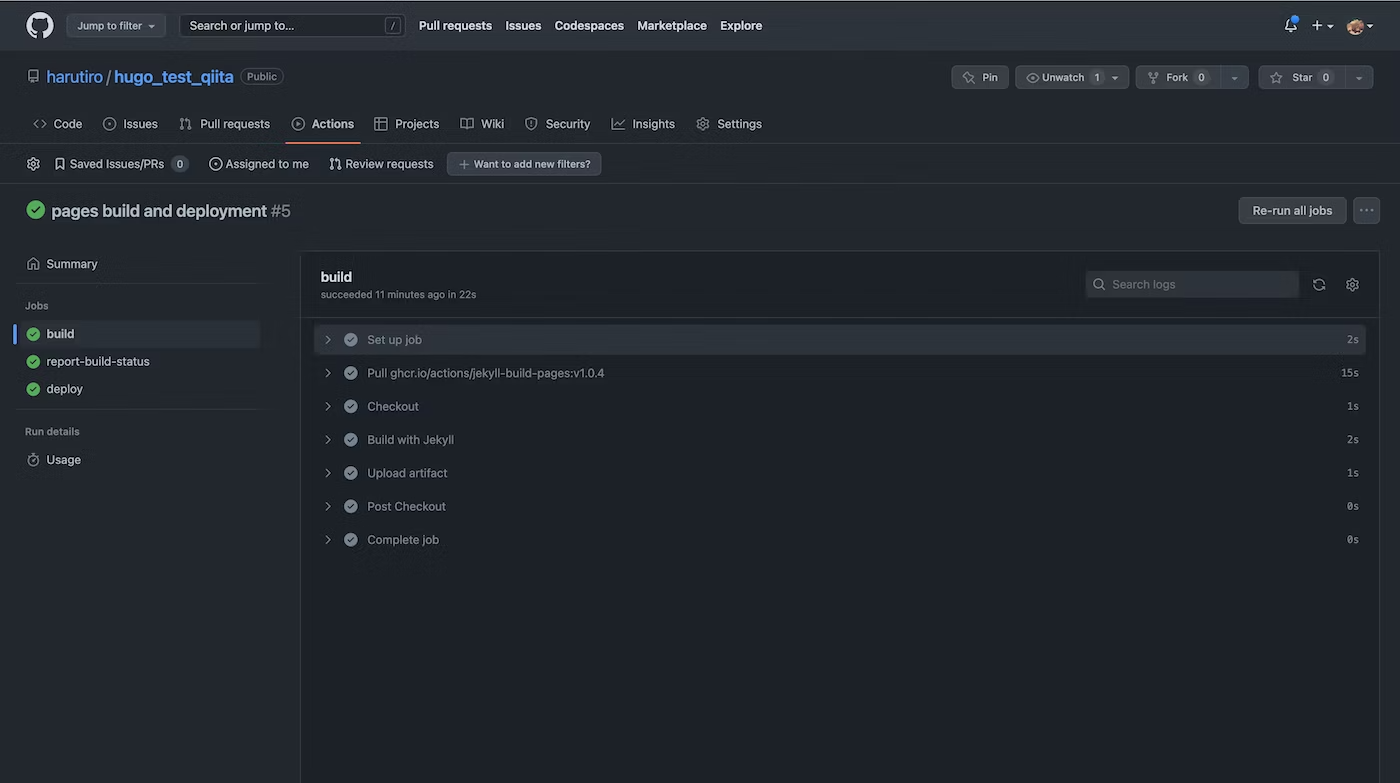
\includegraphics[width=8cm]{./image/02-chap6/git4.png}
    \caption{デプロイが始まった様子}
    \label{chap6-pages2-image}
  \end{figure}

  うまくいった場合、設定したbaseURLの場所に行くとうまく表示されているはずです。

  \begin{figure}[H]
    \centering
    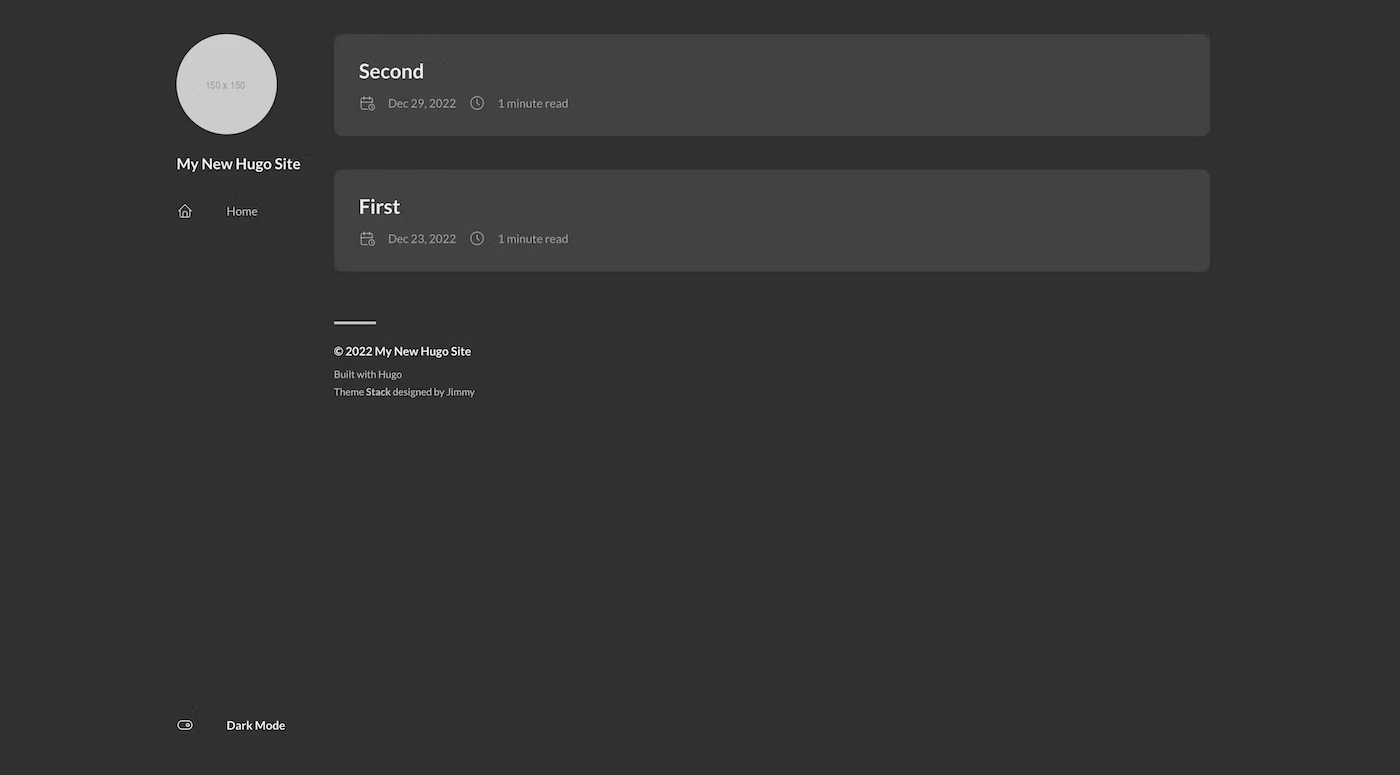
\includegraphics[width=8cm]{./image/02-chap6/view_hugo.png}
    \caption{公開がうまくいった様子}
    \label{chap6-pages3-image}
  \end{figure}



